\chapter{Introduction} \label{cha:intro}
This chapter introduces some of the necessary background required for the rest of this thesis.  First, a general overview of the field of Visualization is provided with its benefits, drawbacks, and dangers for providing context to the rest of the work.  Second, a commonly used version of the visualization pipeline is introduced, elaborating on some of its relevant internal attributes.  The third section presents a small overview over interaction design and its requirements regarding the design of systems where it is essential to have a human-in-the-loop approach.  The last section reviews the literature and elaborates on the fundamentals of user evaluations that seek to answer the question whether novel visualization or interaction techniques are more effective than previous methods.

This chapter is not exhaustive by any means and the inclined reader searching for more detailed information is referred to a great selection of books, such as Preim and Bartz~\cite{preim2007visualization}, Preim and Botha~\cite{preim2013visual}, or Engel~\etal~\cite{engel2006real} to name only a few.

\section{Visualization} \label{cha:intro:vis}
Throughout the years, there have been many attempts at finding a universally accepted definition of \emph{Visualization}.  Card~\etal~suggested that Visualization is ``the use of computer-supported, interactive, visual representations of data to amplify cognition''~\cite{card1999readings}, while other definitions focus more on the interplay between generated imagery and the process of subjective visualization in each person [citation needed], or generalize the concept of visualization to non-visual phenomana as well [citation needed].  While these definitions vary widely, their commonality is the focus on a human observer and the fact that a visualization is created for and by a human, which inherently requires understanding of human physiology.  Furthermore, the field of visualization was started as, and continues to be, a reaction to the data explosion occurring in other fields~\cite{lorensen2004death}, as a means to make sense of the vast quantities of data that these fields regularly generate and that exceed the human capacity.

One potential avenue for distinction, the separation between \emph{explorational} and \emph{presentational} use cases, was put forward, among others, by van Wijk~\cite{van2005value}.  This is addressed and elaborated in a later chapter (Chapter~\ref{cha:contributions}) and forms the basis of the contributions in this thesis.  At the heart is the realization that visualization can be aimed at different audiences and must adapt accordingly in order to be efficient and effective.  Any visualization that does not take the intended audience into account, including their prior knowledge and expectations, fails.

Card~\etal~\cite{card1999readings} and many others often separate the field of visualization into at least three categories, \emph{Scientific Visualization}, \emph{Information Visualization}, and \emph{Visual Analytics}.  

\paragraph{Scientific Visualization} is characterized by the use of data sources with an inherent physical and spatial component.  Data traditionally attributed to Scientific Visualization comes in the form of, for example, simulations or datasets in which the spatial relationship is trivially given.

\paragraph{Information Visualization} usually deals with abstract data that does not need to possess an innate spatial component.  Techniques from this part are typically high-dimensional and multi-variate.

\paragraph{Visual Analytics} places heavier focus on the analytical reasoning and the interaction modes in order to produce insight into the data rather than the source of the data itself.

\noindent Tory~\etal~\cite{tory2002model} pointed out that the required use of words such as ``usually'', ``typically'', or ``traditionally'' hints at a problem with this type of classification.  For once, it is not always possible to delineate differences between the categories even in the most trivial applications~\cite{rhyne2003information, weiskopf2006scivis}.  More complicated applications almost always use reseach from two or all three of these categories, increasing the difficultly of separation.  From an application domain's view point, the distinction between different fields might not even be noticable or relevant.  In their work, Tory~\etal~provide a more nuanced \emph{model-based taxonomy} that is based on the model of the data rather than the data itself.  Rather than using a taxonomy that is based on the description of the data, they propose a taxonomy that is based on the way the data is used inside the visualization system and differentiates between \emph{continous} and \emph{discrete} data, regardless of whether the data itself is abstract or spatial.  This lack of separation between the categories is used in this thesis as they are used to solve the same kinds of problems, displaying data to a human to facilitate insight, utilizing different tools and ``at this level there is much more they share than what separates them''~\cite{van2005value}.

\subsection{Benefits} \label{cha:intro:vis:benefits}
As mentioned in the previous chapter, humans are exceptionally well evolved to interpret the information contained in images.  This is exemplified by the popular quote that ``a picture is worth a thousand words'', meaning that it is significantly easier for humans to ingest information visually rather than through textual description.  Throughout many psychological studies [citation needed] it has been shown that there are two classes of problems.  On the one hand, there are problems that can be solved more efficiently by computers, such as searching large databases and algorithms that typically operate on a map-and-reduce scheme.  On the other hand, there are problems solved better by humans, such as pattern recognition, hypothesis forming, and others [citation needed?].  Visualization, being placed on the boundary between these two problems, can utilize the respective strengths of both computers and humans through a close integration.

\subsection{Limitations} \label{cha:intro:vis:limitations}
One of the important limiting factors influencing each visualization is its subjectiveness.  According to van Wijk, the benefit of using a visualization depends on ```the specification [$\cdots$], the perceptual skills of the observer, and the a priori knowledge of the observer''~\cite{van2005value}.  This is yet another reason why close collaboration between the visualization designer and the domain expert is of fundamental importance, as the design process has to take the experts knowledge into account.  Lorensen elaborated on the potential problems for the visualization community if this collaboration does not occur~\cite{lorensen2004death}.  Another direct consequence of this subjectiveness is that the reproducibility of a visualization is limited to similar consumers.  A visualization system that is designed for experts in a field is totally useless when the same data should be explained to a general public.  

Another aspect of the a priori knowledge that is often overlooked is a dependence on cultural background.  Whereas knowledge-based prior information can be easily assessed, it is much harded to assess cultural bisases.  Some of these cultural differences can be benign, such as the Western tendency to associate movement across a red-green color scale with an increasing value, whereas East Asian cultures would associcate this with a decreasing value, due to the flipped association between the red and green colors.  Other differences can be seen in Figure~\ref{fig:intro:vis:lego}, which displays characters from eight popular cartoon series built from Lego blocks and can be seen as a form of visualization.  Viewed in a culture that is completely unfamiliar with these characters, however, it becomes easy to see that this visualization will be unable to produce any meaningful results.

\begin{figure}
  \centering
  \fbox{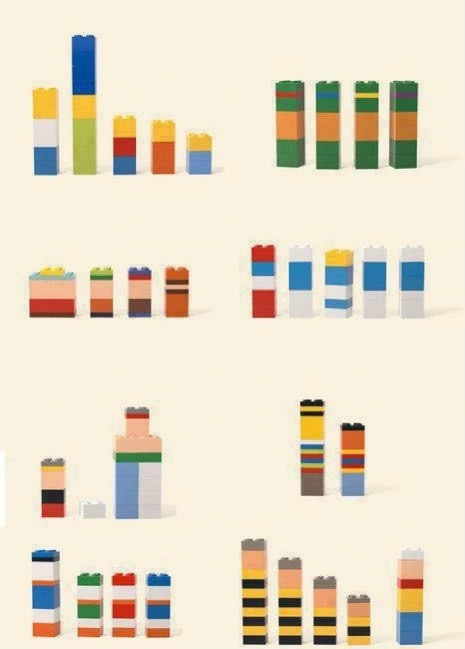
\includegraphics[width=\textwidth]{figures/intro/lego.jpg}}
  \caption{A collection of advertisement images representing cartoon characters. With the required cultural background, deciphering these visualizations is impossible. Image copyright by Lego. Reprinted with permission.}
  \label{fig:intro:vis:lego}
\end{figure}

\subsection{Dangers} \label{cha:intro:vis:dangers}
Besides the immense benefits that visualization can provide for supporting data interpretation and hypothesis testing, there are also aspects where the misuse of visualization can be dangerous to the knowledge increase.  One obvious aspect that is outside the scope of this work is the use of visualization to deliberately mislead the audience.  Even without a deliberate attempt, there are many pitfalls that need to be considered when designing a visualization.  Another danger of the use of visualization is exemplified in the quote from van Wijk saying that ``visualization should not be used to verify the final truth, but rather to inspire to new hypotheses, to be checked afterwards''.  Verifying truths, rather than inspiring hypotheses cna easily lead to confirmation biases that might lead experts to draw faulty conclusions.  Naturally, this danger can only occur in the initial exploration stages of a visualization and can be mitigated when a visualization system is matured and applied to many of the same types of datasets; nevertheless, it is an important aspect to consider during the design process.  The remaining dangers fall into two categories, \emph{showing incorrect information} and \emph{showing information incorrectly}. The first category can occur if visualization designers do not stay true to the data of the expert by, for example, applying smoothing to inherently concrete data sets, not handling outliers correctly in a filtering operation, or not considering missing data in real world datasets.  For the domain expert it becomes increasingly difficult to differentiate missing data from outliers in, for example, a simulation, thus eroding the expert's trust in a visualization system.  In the second category, color maps play a huge role.  Using ill-suited color maps it is trivially possible to highlight or hide structures in the data without informing the expert.  One example if this is the continued use of the rainbow color map in science publications even though it has been shown to be inferior to other color maps~\cite{borland2007rainbow}.



\section{Visualization Pipeline} \label{cha:intro:vp}
\begin{figure}
  \centering
  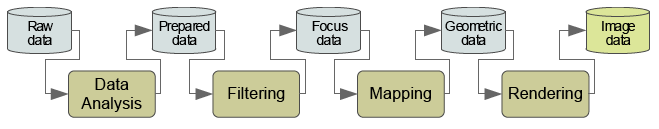
\includegraphics[width=\textwidth]{figures/intro/pipeline.png}
  \caption{One common version of the visualization pipeline as described by Dos Santos and Brodlie. The raw data is transformed multiple steps until an image is generated that can be used by the user to gain insight.  The ability for the user to control each part of the visualization pipeline is at the heart of the human-in-the-loop methodology.}
  \label{fig:intro:vp}
\end{figure}

Figure~\ref{fig:intro:vp} shows a schematic overview of the workflow employed by visualization techniques.  All visualization research attempts to improve one or more of these stages in the pipeline.  The pipeline used was first described by Haber and McNabb~\cite{haber1990visualization} and later extended by Dos Santos and Brodlie~\cite{dos2004gaining} and consists of four transformations that are successively applied to the incoming data.  For a complete description of the visualization pipeline at its variations, we refer to the two original works or by a survey about the development of the visualization pipeline by Moreland~\cite{moreland2013survey}.

The pipeline starts with the \emph{Raw data} that is acquired from measurements or simulations.  This data is processed by the initial \emph{Data analysis}, which consists of data smoothing, interpolation, or the removal of outliers.  In the \emph{Filtering} step, the data is reduced with respect to the requirements of the specific task that is to be solved, for example thresholding, levels-of-detail selection, or segmentation.  This \emph{Focus data} is then used converted in the \emph{Mapping} stage into what Haber and McNabb referred to as Abstract Visualization Objects; an imaginary object that contains the visualization-relatred attributes, such as color, geometry, or texture.  The final step, \emph{Rendering} uses these abstract representations and generates a final image.  It is only in this last step, where the details of a rendering framework, such as OpenGL, are used extensively~\cite{segal2016opengl}.

One important aspect for the design of visualization application systems, that was not fully accounted for in the original visualization pipeline, is the feedback from the user into the various transformation stages.  While it was always possible to change the parameters of the \emph{Rendering} or \emph{Mapping} stages by, for example, changing the camera position, or changing the color attributes of the Abstract Visualization Objects of the \emph{Geometric Data}, the focus of interactivity for the other steps of the pipeline was introduced later with increasing distance from the user.  One of the last feedback loops, Computational Steering, was described by Mulder~\etal~\cite{mulder1999survey}, where the visualization user is able to directly influence the gathering of the \emph{Raw Data} with minimal delay.  Closing this feedback loop leads to the biggest gain in insight as the user can, in the example of simulations, directly understand the influence of parameter changes and can thus gain a deeper understanding of the origin of the data.

\begin{figure}
  \centering
  \fbox{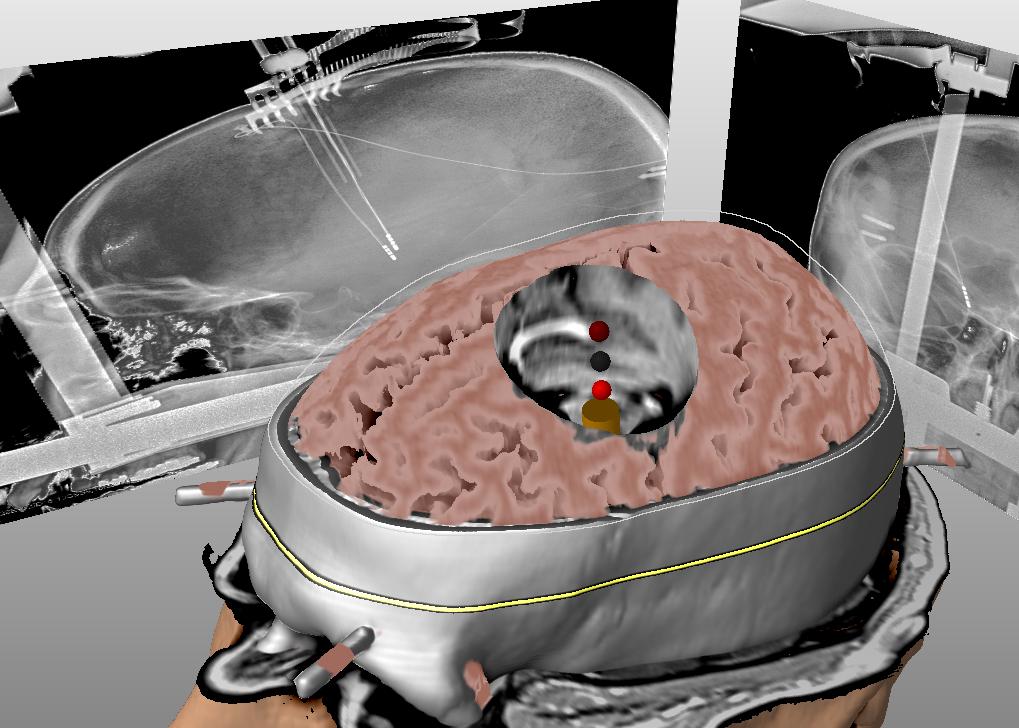
\includegraphics[width=0.5\textwidth]{figures/intro/magicmirror.png}}
  \caption{One example of a multiview visualization, a \emph{Magic Mirror}, where X-ray scans of a patients are shown projected to the sides of a combined volumetric rendering.}
  \label{fig:intro:mm}
\end{figure}

Another important aspect of the visualization pipeline that is hidden from the pipeline depicted in the figure is the possibility of pipeline branching.  Multiview visualization systems provide multiple simultaneous views on different aspects of the data.  One example of these techniques is a magic mirror~\cite{konig1999multiple} as shown in Figure~\ref{fig:intro:mm} that presents different aspects of the underlying data are shown projected to the sides of a surrounding cube.  In a multiview systems, separate branches of the pipeline handle these different views that are ultimately merged in the \emph{Rendering} step.  There exists a large amount of research on techniques dealing with multiview systems, such as brushing or linking~\cite{tory2003mental}.

\subsection{Data Acquisition} \label{cha:intro:vp:da}
Regardless of the exact composition of the visualization pipeline, it always has to start with data that is either collected from the real world or generated by simulations.  While in the abstract, the specific form and shape of the data does not influence the visualization pipeline, concrete systems require knowledge about the origin and characteristics of specific data sources.  This section will elaborate on some of the attributes that are important for the contributions that are included in this thesis.

\subsubsection{Dimensionality} \label{cha:intro:vp:da:dimensionality}
Unfortunately, the word \emph{dimensionality} is overloaded many times in Visualization.  For this section, dimensionality refers to the number of values stored at each location in the dataset, rather than the number of dimensions of the dataset itself.  For the purposes of this work a taxonomy, for example as provided by Shneiderman~\cite{shneiderman1996eyes}, is used that describes data as \emph{scalar}, \emph{vector}, \emph{tensor}, or \emph{multi-dimensional}.  The difference between a \nD{3} and a vector dataset is that a vector has additional information that can be used to restrict the generation of Abstract Visualization Objects.

In addition, each of categories can also be \emph{time-varying}.  While there have been many techniques that efficiently deal with time-varying datasets, for example time-space partitioning trees~\cite{shen1999fast}, efficient handling of these datasets has not been the focus of this thesis.  As such, this work handles the temporal dimension analogous to the already existing spatial dimensions and, thus, a time-varying datasets as an ordered series of single timestep datasets.

\subsubsection{Data Sources} \label{cha:intro:vp:da:sources}
One of the hallmarks of Visualization is that it has to represent and enabled access to real world data.  There are countless potential sources of these datasets and trying to enumerate them would exceed the scope of any single work.  Instead, this section is presenting a brief overview of the different data modalities and their data acquisition techniques that are being utilized in the contributions section.

\paragraph{X-Ray. } X-Ray radiation was discovered by Wilhelm R\"ontgen in 1896~\cite{Rontgen1896xray} and was quickly developed into a viable imaging technique.  A \emph{source} emits x-ray radiation which passes through the medium that is to be imaged.  Based on the constituent materials absorption coefficients, varying amounts of radiation is absorbed when passing through the object.  A photographic plate at the other end of the object displays the incoming x-ray intensity and thus reconstructs a picture of the object.  The limitation with this technique is that it is limited to a single \nD{2} projected image of the object in question and can thus not be easily used for a \nD{3} reconstruction.

\paragraph{Computed Tomography. }  A Computed Tomography (CT) scanner works similar to an x-ray detector, where the source and the electronic detector are rotating around the object that is to be imaged.  Throughout this motion, many images are taken by the scanner, which are then later reconstructed into a \nD{3} representation of the object in question.  The Nobel Prize for Physiology or Medicine was awarded to Godfrey Hounsfield and Allan McLeon Cormack in 1979 for their development of this machine~\cite{Hounsfield1980computed}.  Both spatial and temporal resolution of the scanner has since been improved by multiple orders of magnitude, enabling current machines to perform full-body scans of patients in only a few seconds, or provide the ability to scan a smaller area of interest many tens of times per second, thus extending the available information from the structure aspect into the functional domain.  In human patients, the x-ray radiation is most pronounced in skeletal tissue compared to soft tissue, this imaging modality is most widely used to study bone structure while not being able to highly resolve soft tissue material.

\paragraph{Magnetic Resonance Imaging. }  Magnetic Resonance Imaging (MRI) scanners operate by rapidly manipulating a magnetic and radio-frequency fields that cause the spins of hydrogen atoms.  The radiation emitted by this process is detected by the scanner and used to reconstruct a \nD{3} volumetric representation of the object of study.  Since the signal is based off the availablility of hydrogen atoms, MRI scans exhibit the highest resolution in areas with a high water content, such as soft tissue in human patients, whereas the skeletal structure is not accurately represented~\cite{damadian1971tumor}.  Comparing these attributes to the CT scanner shows that a combination of CT/MRI scanners have the capability of providing a high resolution scanner result for a large part of the human body, thus the combination of these two modalities is often used in practice.

\paragraph{Lidar. }  A Lidar scanner is an active scanner that uses light to a similar effect as radar uses radio waves.  By emitting laser light into the environment and measuring the time it takes for the reflected light to arrive back at the detector, it is possible to create a \nD{3} line-of-sight representation of the area surrounding the scanner.  These measurements can be used to create a high-resolution \nD{3} model of, for example, humans or building structures.  Combining a Lidar scanner with other scanning types, it becomes possible to not only detect the presence or absense of an obstacle, but also measure other physical attributes, for example surface temperature or velocities.  One important use case for lidar scanners are autonomous vehicles that can use the information from lidar to generate an accurate, real-time \nD{3} local environment that can be used for navigation, locomotion, and location.

\paragraph{Simulations. }  The previous modalities generate data through physical processes and thus create a virtual representation of said object which can then be visualized.  Simulations, on the other hand, operate by utilizing a minimal set of physical preconditions and trying to recreate the physical world virtually and thus enabling us insight into areas that would either be infeasible or impossible to investigate directly.  The results of these recreations are highly varying such as simulations of plasma interactions through the simulations of weather phenomen\ae .  An important distinction between the \emph{image-like} modalities and simulations arises in the form of noise that is introduce into the data.  Whereas simulations have the potential to have a very low signal-to-noise ratio, any image-like modality will always have some form, or multiple forms, of noise attached to the signal.

\subsubsection{Grids} \label{cha:intro:vp:da:grids}
There is a variety of methods to structure the data acquired by the aforementioned modalities.  This section will introduce a subset of possible data layouts with a focus on the data types that are utilized in this thesis.  This is by no means a complete reference as each specific problem domain can demand its own data representation.

\paragraph{Point Cloud. }  Point cloud data is the least structured of these data types and consists of, potentially multi-dimensional, measurements in a \nD{2} or \nD{3} space.  A Lidar scanner are a prime example of a modality that generates unstructured point cloud.  Point clouds, due to their unstructured storage, are notoriously difficult to handle and thus pose unique visualization challenges, such as handling transparency, occlusion, and the need for efficient rendering techniques.

\paragraph{Cartesian. }  Multidimensional Cartesian grids are the most widely used form of structured data, with \nD{3} grids being the most applicable to this thesis.  The uniform storage of this grid makes it possible to efficiently handle a large amount of data, for example by using isosurface rendering or \emph{direct volume rendering}.  The ubiquitious nature of Cartesian grids also provides a major drawback.  Since it is the \emph{de facto} standard data format, it is often used in areas that are not filling an $n$ dimensional space or where an adaptive resolution is necessary and thus lead to oversampling.  This results is suboptimal storage requirements for Cartesian data sets in these cases where an adaptive grid or a different underlying geometry would be better suited.

\paragraph{Spherical. }  One non-Cartesian grid structure that is used in this work is a grid based on spherical or polar coordinates.  Simulations of the Sun inside our solar system produce higher resolution closer to the origin and automatically possess a spherical symmetry which can be utilized to minimize the conversion efforts and storage capacity.  In these cases, a spherical data set is a \nD{3} volume, where each axis represents the three spherical coordinate axis, $r$, $\phi$, and $\theta$ respectively.  When applying rendering techniques, such as \emph{direct volume rendering} to this volume interesting characteristics, such as automatic adaptive sampling, can be observed.

\subsection{Direct Volume Rendering} \label{cha:intro:vp:dvr}
Most of the work presented here deals with \nD{3} data sets for which \emph{direct volume rendering}~(DVR) is a very well-suited and well-established rendering algorithm that was derived from simplifying ray tracing algorithms and thus making it possible to be computed at interactive frame rates.  Traditionally, DVR uses a simple emission/absorption model that assumes that the volume is composed of small particles that each have the ability to emit and absorb light~\cite{levoy1988display, drebin1988volume, sabella1988rendering}.  For a specific position $\vec{x_0}$ in the volume and a virtual camera location $\vec{x_c}$, light is emitted, partially absorbed, and combined with the ambient background light to form an image.  The mathematical formulation of the incoming radiance $I$ was first described by Max~\cite{max1995optical, max2010local} as:
\begin{equation}
I(\vec{x_c}) = \underbrace{I_0\left( \vec{x_0} \right) T\left( \vec{x_0}, \vec{x_c} \right)}_{\textrm{Background}} + \int_\vec{x_c}^\vec{x_0}  \underbrace{T(\vec{x_c}, \vec{x})}_{\textrm{Attenuation}} \underbrace{\sigma_\alpha(\vec{x}) I_c(\vec{x}}_{\textrm{Contribution}} \textrm{d} \vec{x},
\label{eqn:intro:dvr}
\end{equation}
\noindent where $I_0$ determines the background illumination, $\sigma_\alpha$ determines whether a sample $\vec{x}$ is emitting or absorbing light and $I_e$ specifies the amount of light contributed at a location $\vec{x}$, attenuated by $T(\vec{x_c}, \vec{x})$.  The attenuation factor is given by:
\begin{equation}
T(\vec{a}, \vec{b}) = \exp \left( -\int_\vec{a}^\vec{b} \tau(\vec{x}) \textrm{d} \vec{x} \right),
\label{eqn:intro:dvr2}
\end{equation}
\noindent with $\tau(\vec{x})$ being the extinction coefficient that defines the occusion of light within the volume.  Equations \ref{eqn:intro:dvr} and \ref{eqn:intro:dvr2} are known as the volume rendering integral.

In practical calculation, the integrals in the volume rendering integral are approximated as Riemann sums with a stepsize $h$ between individual samples.  $h$ can be either a constant value that should be limited by Nyquist's theorem~\cite{shannon1949communication}, or dependent on the encountered data values.  This would lead to implementations of adaptive sampling~\cite{danskin1992fast} or empty space skipping~\cite{yagel1993accelerating}.  These Riemann sums are constructed for each pixel in the rendering window based off the bounding geometry of the volume that is to be rendered.  By rendering the coordinates of the volume's bounding geometry and storing the results, it is possible to generate each pixel's ray and traverse it in the graphics processing unit (GPU)~\cite{kruger2003acceleration}.

\section{Human-in-the-Loop} \label{cha:intro:hitl}
\begin{itemize}
  \item Combination of automated systems and human-in-the-loop; Shows importance of domain expert integration
  \begin{itemize}
    \item Interaction design
    \item \cite{munzner2014visualization} \cite{van2005value} -> Shows importance of domain expert integration
  \end{itemize}
\end{itemize}
